\question{}

\begin{ابجد}
\item \textbf{نادرست}؛ در جستجوی گرافی تمام گره‌هایی که قبلاً از آنها بازدید کرده‌ایم نیز ذخیره می‌شوند تا از بررسی مجدد آنها جلوگیری شود. بنابراین پیچیدگی فضایی\footnote{\lr{Space Complexity}} الگوریتم \lr{DFS} در این حالت از مرتبه $O(b^m)$ می‌باشد.

\item \textbf{درست}؛ طبق تعریف تابع اکتشافی $h$ یک‌نوا است اگر:
\[ \forall A, B: h(A) - h(B) \leq \mathrm{cost}(A \to B) \]
حال اگر دو تابع اکتشافی $h_1$ و $h_2$ یک‌نوا باشند، به سادگی می‌توان نتیجه گرفت که:
\begin{align*}
    h_1(A) - h_1(B) & \leq \mathrm{cost}(A \to B) \\
    h_2(A) - h_2(B) & \leq \mathrm{cost}(A \to B)
\end{align*}
با جمع دو رابطه بالا داریم:
\[ (h_1 + h_2)(A) - (h_1 + h_2)(B) \leq 2 \times \mathrm{cost}(A \to B) \]
با تقسیم طرفین بر $2$ نتیجه می‌شود:
\[ \forall A, B: \left(\frac{h_1 + h_2}{2}\right)(A) - \left(\frac{h_1 + h_2}{2}\right)(B) \leq \mathrm{cost}(A \to B) \]
بنابراین $\frac{h_1 + h_2}{2}$ یک تابع اکتشافی یک‌نوا است.

\item \textbf{نادرست}؛ مثال نقض می‌آوریم. فرض کنید به ازای تابع اکتشافی $h_1$ و دو گره $A$ و $B$ داریم:
\begin{align*}
    h_1(A)                 & = 3 \\
    h_1(B)                 & = 2 \\
    \mathrm{cost}(A \to B) & = 2
\end{align*}
می‌دانیم که $h_1$ یک‌نوا هست و رابطه $h_1(A) - h_1(B) \leq \mathrm{cost}(A \to B)$ صحیح می‌باشد. حال اگر عدد ثابت $c = 3$ را در نظر بگیریم:
\begin{align*}
    h_2(A) & = 9 \\
    h_2(B) & = 6
\end{align*}
اکنون داریم $h_2(A) - h_2(B) = 3 \nleq \mathrm{cost}(A \to B)$ و رابطه مورد نظر دیگر برای گره‌های $A$ و $B$ صادق نیست، پس تابع $h_2$ یک‌نوا نیست.

\item \textbf{درست}: می‌دانیم طبق تعریف به تابع اکتشافی‌ای قابل قبول\footnote{Admissible} گفته می‌شود که:
\begin{align*}
    \forall n, 0 \leq h(n) \leq h^*(n)
\end{align*}
که $h^*(n)$ هزینه واقعی است.
\begin{proof}
    فرض کنید دو هدف قابل دسترس $A$ و $B$ داریم که $A$ بهینه و $B$ غیر بهینه\footnote{suboptimal} است. $n$ یک جد دلخواه $A$ (شامل خود $A$) است؛ می‌خواهیم نشان دهیم که $n$ زودتر از $B$، از \lr{fringe} خارج می‌شود. از سه مورد زیر استفاده می‌کنیم:
    \begin{enumerate}
        \item $g(A) < g(B)$؛ چون $A$ هدف بهینه، و $B$ غیر بهینه است.
        \item $h(A) = h(B) = 0$؛ چون تابع $h$ قابل قبول است.
        \item $f(n) \leq f(A)$؛ به این شکل نشان داده می‌شود:
              \begin{align*}
                  h(n) \leq h^*(n) \Rightarrow & g(n) + h(n) \leq g(n) + h^*(n) \\
                  \Rightarrow                  & f(n) \leq g(A)                 \\
                  \xRightarrow{h(A) = 0}       & f(n) \leq f(A)
              \end{align*}
    \end{enumerate}
    اکنون از این سه مورد استفاده می‌کنیم:
    \begin{align*}
        \text{1 و 2} \Rightarrow g(A) + h(A) < g(B) + h(B)       \Rightarrow & f(A) < f(B)               \\
        \xRightarrow{\text{3}}                                               & f(n) < f(B) \quad (\star)
    \end{align*}
    چون از ابتدا فرض کرده بودیم که $n$ یک جد دلخواه $A$ (شامل خود $A$) هست، طبق رابطه ($\star$) نتیجه می‌گیریم که تمام اجداد $A$ از جمله خودش، پیش از $B$ بسط داده می‌شوند؛ پس نتیجه می‌گیریم که در این حالت الگوریتم $A^*$ بهینه است.
\end{proof}

\item \textbf{نادرست}؛ الگوریتم \lr{Local Beam Search} با $k=1$، همواره تمام همسایه‌های حالت فعلی را تولید کرده و سپس بهترین گزینه بین آنها را انتخاب می‌کند؛ بنابراین اگر تمام همسایه‌ها بدتر از حالت فعلی باشند، الگوریتم به ناچار بهترینِ آن‌ها را (که نسبت به حالت فعلی بدتر است) انتخاب می‌کند. \\
در مقابل الگوریتم \lr{Simulated Annealing} هر بار به طور تصادفی یکی از همسایه‌ها را انتخاب می‌کند: اگر این همسایه بهتر از حالت فعلی باشد، انتخاب می‌شود. اما اگر بدتر باشد، با احتمالی انتخاب می‌شود که این احتمال با کاهش دما کم می‌شود. به طور خلاصه هنگامی که دما به صفر میل می‌کند، الگوریتم \lr{SA} همسایه‌ای که بدتر از حالت فعلی باشد را انتخاب نمی‌کند، و از طرفی همسایه انتخاب شده هم لزوما «بهترین» همسایه ممکن نیست.

\item \textbf{نادرست}؛ الگوریتم \lr{BFS} در طول اجرای خود هر گره را حداکثر یک بار بسط می‌دهد. در مقابل، الگوریتم \lr{IDS} هر بار که حد عمق (\lr{limit}) جدیدی تعریف می‌کند، جستجو را مجدداً از ریشه درخت آغاز کرده و تمام گره‌های سطوح قبلی را دوباره بسط می‌دهد. \\
به همین دلیل، گره‌های سطوح بالاتر چندین بار (به عنوان مثال، گره ریشه $d+1$ بار) باز می‌شوند. در نتیجه، تعداد کل گره‌های بسط‌یافته در \lr{IDS} همواره اکیداً بیشتر از \lr{BFS} است (هرچند مرتبه مجانبی هر دو $O(b^d)$ می‌باشد).

\item \textbf{درست}؛ می‌دانیم که الگوریتم \lr{UCS} همواره گره با کمترین هزینه را از \lr{fringe} خارج می‌کند. حال اگر یال با هزینه 0 داشته باشیم، ممکن است الگوریتم در یک حلقه گیر کرده و هیچ گاه خاتمه نیابد. به عنوان مثال فرض کنید هم از گره $A$ به گره $B$ یال داریم و هم از گره $B$ به گره $A$، و هزینه هر دو یال نیز صفر است. همچنین فرض کنید در این مسئله هزینه تمام اکشن‌های دیگر بیشتر از صفر باشد. در این صورت اگر الگوریتم به یکی از این دو گره برسد، همواره یال با هزینه صفر را انتخاب می‌کند و هیچ گاه از این حلقه خارج نمی‌شود. \\
البته باید توجه کنیم که این مثال برای \lr{UCS} در حالت جستجوی درختی درست است. اگر بخواهیم از الگوریتم در جستجوی گرافی استفاده کنیم، از آنجا که در این حالت الگوریتم لیست گره‌های بسط داده شده را نگه می‌دارد (\lr{closed set}) امکان ندارد که در دوری با تعداد گره محدود گیر کند؛ در این روش تنها حالتی که امکان دارد گره در یک دور گیر کند، این است که یک دنباله از گره‌ها داشته باشیم که هزینه بین هر دو گره متوالی 0 باشد؛ در این صورت دیگر فضای مسئله متناهی نیست. (این موضوع منافاتی با صورت مسئله ندارد، چون ممکن است که در این فضا یک پاسخ متناهی داشته باشیم.)

\item \textbf{درست}؛ برای اثبات یک‌نوا بودن تابع اکتشافی $h$ باید نشان دهیم به ازای دو گره دلخواه \lr{A} و \lr{B}، که از \lr{A} به \lr{B} مسیری وجود داشته باشد:
\begin{align*}
    h(A) - h(B) \leq \mathrm{cost}(A \to B)
\end{align*}
یا به طور معادل:
\begin{align*}
    h(A) \leq \mathrm{cost}(A \to B) + h(B)
\end{align*}
\begin{proof}
    از یک‌نوا بودن $h_1$ و $h_2$ نتیجه می‌گیریم که به ازای هر دو گره دلخواه \lr{A} و \lr{B}، که از \lr{A} به \lr{B} مسیری وجود داشته باشد، داریم:
    \begin{align*}
        h_1(A) \leq \mathrm{cost}(A \to B) + h_1(B) \qquad & \text{(1)} \\
        h_2(A) \leq \mathrm{cost}(A \to B) + h_2(B) \qquad & \text{(2)}
    \end{align*}
    تابع اکتشافی $h = \min(h_1,h_2)$ را بررسی می‌کنیم.
    می‌دانیم که:
    \begin{align*}
        h(B) = h_1(B) \lor h(B) = h_2(B)        \qquad & \text{(3)} \\
        h(A) \leq h_1(A) \land h(A) \leq h_2(A) \qquad & \text{(4)}
    \end{align*}
    بنابراین:
    \begin{align*}
        \text{(4)} \xRightarrow{\text{(1) , (2)}} {\left\{\begin{aligned}
                                                                  h(A) \leq \mathrm{cost}(A \to B) + h_1(B) \\
                                                                  h(A) \leq \mathrm{cost}(A \to B) + h_2(B)
                                                              \end{aligned}\right.} \xRightarrow{\text{(3)}} h(A) \leq \mathrm{cost}(A \to B) + h(B)
    \end{align*}
    بنابراین تابع اکتشافی $h$ یک‌نوا است.
\end{proof}

\item \textbf{نادرست}: به طور کلی با افزایش $k$ در الگوریتم \lr{Local Beam Search} حالت‌های بیشتری بررسی می‌شوند و شانس گیر کردن در نقاط \lr{local maximum} یا نواحی \lr{flat} کمتر می‌شود. اما با افزایش $k$، تعداد همسایه‌هایی که باید در هر حالت محاسبه شوند نیز بیشتر می‌شود که در این حالت اجرای هر مرحله از الگوریتم مدت زمان بیشتری طول می‌کشد و ممکن است پیش از رسیدن به حالت هدف، زمان اجرای الگوریتم تمام شود. همچنین در هر مرحله باید همسایه‌های $k$ حالت فعلی ذخیره شوند تا بتوانیم $k$ تای بهتر را از بین آنها انتخاب کنیم. اگر تعداد همسایه‌ها خیلی زیاد شود، ممکن است به محدودیت حافظه بخوریم و الگوریتم متوقف شود.

\item \textbf{نادرست}: مثال نقض می‌آوریم. به این شکل توجه کنید:
\begin{latin}
    \begin{center}
        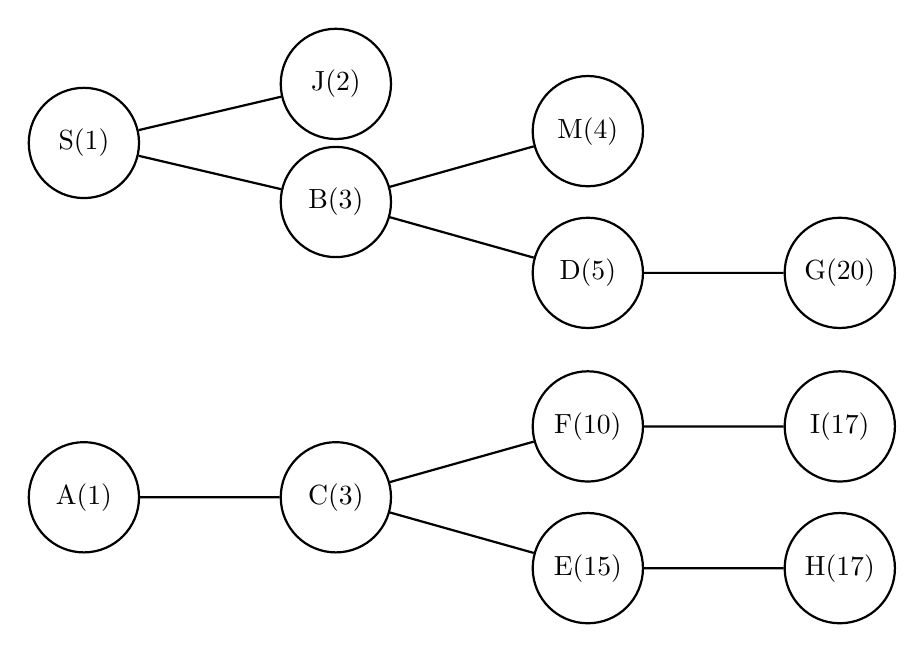
\begin{tikzpicture}[
                grow=right,
                level distance=3.2cm,
                level 2/.style={sibling distance=1.8cm},
                every node/.style={
                        draw, thick, circle,
                        minimum size=1.4cm,
                        inner sep=0pt,
                        align=center
                    },
                edge from parent/.style={draw, thick}
            ]

            \node at (0, 2) {S(1)}
            child {node {B(3)}
                    child {node {D(5)}
                            child {node {G(20)}}
                        }
                    child {node {M(4)}}
                }
            child {node {J(2)}};

            \node at (0, -2.5) {A(1)}
            child {node {C(3)}
                    % Bottom branch
                    child {node {E(15)}
                            child {node {H(17)}}
                        }
                    % Top branch
                    child {node {F(10)}
                            child {node {I(17)}}
                        }
                };

        \end{tikzpicture}
    \end{center}
\end{latin}
در این مثال هر گره، یکی از حالت‌های کامل\footnote{Complete} مسئله است و مقابل اسم هر یک، مقدار تابع \lr{fitness} به ازای آن نوشته شده. همچنین حالت‌های همسایه با یال به هم متصل شده‌اند. هدف، پیدا کردن حالت با بیشینه مقدار تابع \lr{fitness} است که در این مثال همان حالت $G$ می‌باشد. \\
در این مثال، الگوریتم \lr{Hill Climbing} با شروع از حالت $S$، به ترتیب به گره‌های $B$، $D$ و در نهایت به حالت هدف $G$ می‌رسد. الگوریتم \lr{Local Beam Search} با $k=2$ که از حالت‌های $S$ و $A$ شروع می‌کند، در مرحله اول گره‌های $B$ و $C$، سپس گره‌های $F$ و $E$، و در نهایت حالت‌های $I$ و $H$ را انتخاب کرده و بدون رسیدن به حالت هدف $G$، خاتمه می‌یابد.

\end{ابجد}